\documentclass[letter,11pt,oneside]{article}

%%% (occur "\\(\\\\[a-z]*section\\|appendix\\|input\\|\\<include\\>\\)")

%%\documentclass[11pt,twocolumn]{article}
%%\usepackage[inline]{asymptote}   %% Inline asymptote diagrams
%%\usepackage{wglatex}             %% Use this one and kill others.
\usepackage{color}               %% colored letters {\color{red}{{text}}
\usepackage{fancyhdr}            %% headers/footers
%%\usepackage{fancyvrb}            %% headers/footers
\usepackage{datetime}            %% pick up tex date time 
\usepackage{lastpage}            %% support page of ...lastpage
\usepackage{times}               %% native times roman fonts
\usepackage{textcomp}            %% trademark
\usepackage{amssymb,amsmath}     %% greek alphabet
\usepackage{parskip}             %% blank lines between paragraphs, no indent
\usepackage{shortvrb}            %% short verb use for tables
\usepackage{lscape}              %% landscape for tables.
\usepackage{longtable}           %% permit tables to span pages wg-longtable
\usepackage{url}                 %% Make URLs uniform and links in PDFs
\usepackage{enumerate}           %% Allow letters/decorations for enumerations
\usepackage{endnotes}            %% Enhance footnotes/endnotes
\usepackage{listings}            %% Make URLs uniform and links in PDFs
\pdfadjustspacing=1                %% force LaTeX-like character spacing
\usepackage{geometry}            %% allow margins to be relaxed
%%\usepackage{wrapfig}             %% permit wrapping figures.
%%\usepackage{subfigure}              %% images side by side.
\geometry{margin=1in}            %% Allow narrower margins etc.
\usepackage[T1]{fontenc}         %% Better Verbatim Font.
\renewcommand*\ttdefault{txtt}   %% 
%%\usepackage{natbib}   %% bibitems

%% include background image (wg-document-page-background) 

\usepackage{graphicx}            %% Include pictures into a document
%% (wg-texdoc-inserttikz)


\def\documentisdraft{NOTDRAFT}

%% (wg-texdoc-isdraft)
%% (wg-texdoc-insert-fancy-headers)

%%\usepackage[bookmarks]{hyperref} %% Make huperlinks within a PDF
%%\usepackage{makeidx}             %% Make an index uncomment following line
%%\makeindex                       %%.. yeah this one, too. index{key} in text
%%



\definecolor{verbcolor}{rgb}{0.6,0,0}
\definecolor{darkgreen}{rgb}{0,0.4,0}
\newcommand\debate[1]{\textcolor{darkgreen}{DEBATE: #1} \marginpar{\textcolor{red}{DEBATE} }}
\newcommand{\ltodo}[2]{\marginpar{\textcolor{red}{ACTION: #1}\endnote{#2}}}
\renewcommand{\thefigure}{\thesection-\arabic{figure}}
\newcommand{\menu}{\ensuremath{\;\rightarrow\;}}
\newcommand{\dhl}[1]{{\color{verbcolor}{\texttt#1}}}

%%(wg-add-inline-images)  %% add inline images to the mix





%%Begin User Definitions: Hint: ~/.latex.defs and  latex.defs  
%%End User Definitions:
%%(wg-texdoc-adjust-paper-width)
%% (wg-texdoc-insert-hypersetup)



%%%%%%%%%%%%%%%%%%%%%%%%%%%%%%%%%%%%%%%%%%%%%%%%%%%%%%%%%%%%%%%%%%%%%%%%%%%%%


\begin{document}


%% (wg-latex-pretty-title-page)
%% (wg-texdoc-titleblock)

\setcounter{section}{0}
\pagenumbering{arabic}

\ifx\documentisdraft\drafttest
\linenumbers    %%%%%%%%%%%%% DRAFT
\fi


\section{Managing Astronomical Files}

Science damands discipline.

\vspace{-.15cm}
\begin{enumerate}\addtolength{\itemsep}{-0.5\baselineskip}
   \item  You go to the observatory.
   \item  You observe all night.
   \item  You have a collection of raw data from the telescope, together with
a few side files.  Warts blisters and all.

\end{enumerate}

These are big files -- fact of life.

Now best-practices enters the thought process.

Never work on raw data. They should be saved somewhere.
OK there is the archive copy in git.

Now, no matter what, I have 2x the file sizes of disk.

I use 3 directories and a side directory.

\vspace{-.15cm}
\begin{enumerate}\addtolength{\itemsep}{-0.5\baselineskip}
   \item   usw - catalogs, finder image, target list, notes
   \item   RawData - the exact data from observatory, read-only
   \item   PreAnalysis - copied, fixed and reduced RawData (temporary dir)
   \item   Analysis - Container for final products of the night.
\end{enumerate}


I save Analysis. I ignore PreAnalysis as I can reproduce it.
Exactly. (If you can't reproduce it -- get a better process).

At the end:

\vspace{-.15cm}
\begin{enumerate}\addtolength{\itemsep}{-0.5\baselineskip}
   \item   I move to the top of my repository.
   \item   git add . \# Note the dot at the end
   \item   git commit \# editor pops up, I describe the commit
   \item   git push origin master
\end{enumerate}


I am done.

I have the raw data and two copies of my Analysis products.
One in my safe, the other out there to play with.

The size should be exactly the same size as what you are doing
now, with a few files as part of the collaboration.

You do not want to play safely, these are your chances to take.


\subsection{Intermediate files}

\vspace{-.15cm}
\begin{enumerate}\addtolength{\itemsep}{-0.5\baselineskip}
   \item   fix file names
   \item   trim (remove overscan)
   \item   cosmic ray remove
   \item   make masters
   \item   apply masters
   \item   platesolve
   \item   combine
   \item   refer for analysis (copy to permenant Analysis directory)
   \item   remove this dir if I want to.
\end{enumerate}

For one raw file I wind up with..

\begingroup \fontsize{10pt}{10pt}
\selectfont
%%\begin{Verbatim} [commandchars=\\\{\}]
\begin{verbatim} 
t_raw.fits            # trimmed
cr_t_raw.fits         # and cosmic ray cleaned (SPEs in zeros!)
z_cr_t_raw.fits       # and zero subtracted
d_z_cr_t_raw.fits     # and dark subtracted as needed
f_d_z_cr_t_raw.fits   # and flattened
s_f_d_z_cr_t_raw.fits # and platesolved
raw.cat               # extracted info for raw file
combined.fits         # and combined into final product
combined.cat          # extracted info for combined image
\end{verbatim}
\endgroup
%% \end{Verbatim}

I refer for analysis all cat files and the combined files.
I destroy the PreAnalysis directory (OK I have disk space
so it is there for a while). 

Now I:

\vspace{-.15cm}
\begin{enumerate}\addtolength{\itemsep}{-0.5\baselineskip}
   \item  git add .
   \item  git commit (fill in comments)
   \item  git push origin master
   \item  git request-pull v1.0 master
\end{enumerate}


...and head out to the day. My working tree is good. My
archive, on a different computer is up to date.






\section{Using GitHub SAS Spectroscopy Repository}


See Appendix \ref{Started} for software to get started.

The hallmark of collaboration is to assure people are using
the same information and data to reach desired outcomes. 

Git is a 'distributed' management system. Each 'clone' or
repository is unique and stands alone on the system where
it exists. It is identical to the 'bare' repository located
on GitHub except the latest file of a set of archived
files is maintained as a ready-to-use image.

Good habits make these repositories the same approximate size
of the ones you already use.

\subsection{Prepare for clones}

Make a directory (folder) 'somewhere' on your system. This can
be a $100 2T USB drive. 

With the git program installed (again Appendix \ref{Started} for
software to get started), you:

- Use the browser, login to GitHub and find the repository to 'clone'.
- The green-button on the repo lets you get a full zip file, or 
offers the URL for the 'clone'.
- Using the windows gui, (See video) make a clone on your system.


The downsides:
\vspace{-.15cm}
\begin{enumerate}\addtolength{\itemsep}{-0.5\baselineskip}
   \item   Email confusing and no record of changes is maintained
   \item   Dropbox people move large things though their accounts, files
may be lost.
   \item   GitHub - A minimum of 2x the file size on local machine, with
nx for files that are changed.
\end{enumerate}


The upsides:
\vspace{-.15cm}
\begin{enumerate}\addtolength{\itemsep}{-0.5\baselineskip}
   \item   Email - none
   \item   Dropbox - smaller size for a bit/piece of overall project
   \item   GitHub - the environment also has a wiki, some files viewable
in browser (fits not so much).
\end{enumerate}

GitHub is a suite of tools to work with ``git'' repositories. 
See \url{https:/git}

Anytime more than a very few people try to collaborate by sharing code
and data the effort becomes tedious and complex. By having one central
location serve as a ``bulletin board'' the complexity comes down 
dramatically. A bulletin board that serves to track changes,
and provide version control amplifies outcomes of collaboration.
GitHub provides something that is more than a forum. It includes
'the' official version of spreadsheets, code, images and documents.
It provides a 'wiki' for links etc.

Participants are allowed to edit the content directory. We are
a 'collaboration' after all.

the GitHub combined with Zoom offers this community powerful ways
to interact in a timely fashion. 

Woody Sims and I used a 'git' based system to coordinate a series of
observations, tests and exploration of alternatives in imaging and
spectroscopy using BitBucket's suite. However, we found the suite with
GitHub to be much better. Adding Zoom has created a dynamic environment
beyond what is currently available. We even have a classical forum
via google-groups.

The benefits:

\vspace{-.15cm}
\begin{enumerate}\addtolength{\itemsep}{-0.5\baselineskip}
   \item   To join the collaboration, you are given your credentials once
and then you simply copy the entire history to your machine.
   \item   The web-based interface to GitHub allows you to see most files
directly via the browser. 
   \item   GUI tools come with git. Git-gui is easy to use.
   \item   Massivly complex operations with branching and other concepts found
in software engineering exist but may be ignored, left dormant until 
needed.
\end{enumerate}



\begin{quote}
As with most other distributed version-control systems, and unlike
most client--server systems, every Git directory on every computer is
a full-fledged repository with complete history and full
version-tracking abilities, independent of network access or a central
server. \footnote{Chacon, Scott (24 December 2014). Pro Git (2nd
  ed.). New York, NY: Apress. pp. 29--30. ISBN 978-1-4842-0077-3}
\end{quote}

\subsection{Getting Started}

\appendix
\renewcommand \thesection{\Alph{section}}

\section{Basic Steps (Big Picture)}

Your copy of the repository is called a 'clone'.

You can put clones anywhere, they only care about 'stuff'
that is under the their directory. They don't put anything
in Windows registry. They maintain their side-notes in
a hidden directory within the clone.

I like to put my clones in one place, a directory simply
called 'git' off my main home directory. 

So, make the git directory (folder) and put your clones there.

We currently have to main clones going:
  SAS\_Specgtrography \\
  SAS\_3DSpectrographs

there will be more -- probably ones devoted to observing campaigns.

\subsection{Get the Program}

- Download and install the 'git' program for your platform(s).
 \url{https://git-scm.com/downloads} and pick the platform.
- Visit our collaboration at GitHub: and get the web url of
the repository. \url{https://github.com/dxwayne/SAS_Spectroscopy.git}
- Using the Git-Gui program (Windows)
  - 
  -

Now the files are in your git folder, under the directory
\dhl{SAS\_Specgtrography/Observations/SampleDatasets/LISA/V694 Mon}


\begin{figure}[h!]
\centering
%%\phantomsection
%%\addcontentsline{toc}{section}{}
%%\caption{} %% \caption{{\tiny{citation}}} 
%%\includepdf[angle=90,width=\textwidth]{}); %% with package pdfpages
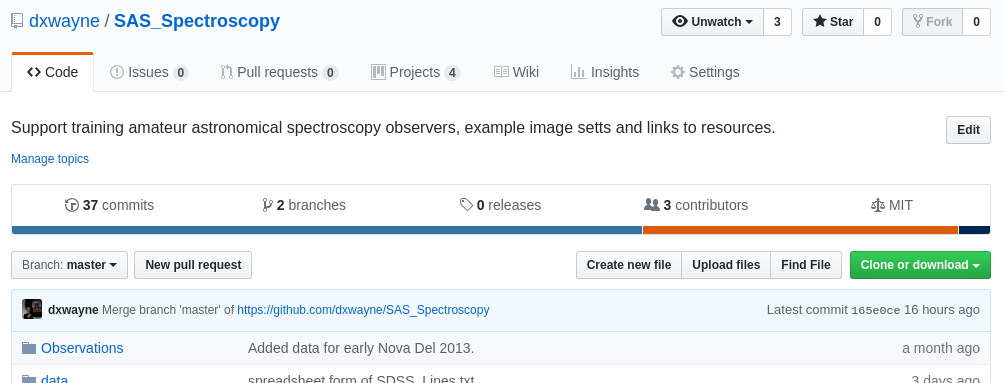
\includegraphics[width=\textwidth]{images/GitHubOverview.png}
\caption{} %% \caption{{\tiny{citation}}} 
\label{figure:}
\end{figure}


%% use a bibitem approach to the references publications etc.
%% (wg-bibitem)

%%\clearpage
%%\addcontentsline{toc}{section}{References}
%%\renewcommand*{\refname}{My Bibliography and References}
%%\bibliographystyle{plain}	% bibliographystyle{apalike} and \usepackage{natbib}
%%\bibliography{MasterBib}	% expects file "MasterBib.bib"


%%\clearpage
%%\addcontentsline{toc}{section}{Index}
%%\printindex %% www.cs.usask.ca/resources/tutorials/latex/notes/toc-index.pdf

%%\begin{thebibliography}{80}
%%\usepackage{natbib}   %% bibitems
%%\end{thebibliography}

% /home/wayne/git/SAS_Spectroscopy/doc/GitHub.tex

%% (wg-texdoc-endnotes)
\end{document}


The hallmark of collaboration is to assure people are using
the same information and data to reach desired outcomes. 

Git is a 'distributed' management system. Each 'clone' or
repository is unique and stands alone on the system where
it exists. A single 'bare' repository can be used as the
central manager for all changes. Multiple people 'clone'
the bare repository as a working repository onto their
machine. 

Changes can be made, erased, tried again until a polished
version is ready to share. It is then 'pushed' to the
remote bare repository -- and other people can 'pull' it
down to bring their copy up-to-date. 

The system tracks pending changes and lets you manage how
to release that data.

The system can be told to ignore certain files or directories.

Where the 'bare' repository resides is up to the agreement
between users. Personally, I use git on a Synology RAID
backup box to hold 'bare' repositories that I don't need
to share with anyone. I use GitHub to manage 'bare' repositories
I do share. They include Phoenix-Asteroids 2013 -- a student
collaboration to observe asteriods. It has been updated once
when JPL changed their interface -- and will be updated in
a few weeks when the do the next update.

GitHub allows me to have 'private' repositories and I can invite
people to work with those data as 'collaborators'. SAS Spectroscopy
is a 'private' reposotory.

In addition to the repository, I get a 'wiki' a private way to
provide basic documentation and administration information.

Many files can be edited directly on the main repo. Every now
and then we make a 'release'. 

One technical thing is each repository maintains a copy of
every file ever commited to the batch. A 'clone' maintains
one additional file -- the toplevel file -- ready for action.
This means twice the file space.

Astronomical Images:

Nobody wants to take the time to understand FITS files. The pro's
know the details but need to be reminded from time to time.

Astronom exposures can be stored as 'raw' data with a 16-bit
unsigned integer for each pixel. This makes the 'raw' image
1/2 the size of a float. So a repository with a archive
and working copy of the file -- well ...

..It is the same size as what you should be doing now.
With a small amount of overhead. 

The rest of the files, docs, occasional jpegs, etc are small
by comparison anyway.
